\documentclass[a4paper, 11pt]{article}
\usepackage{geometry}
\geometry{letterpaper, margin=1in}
\usepackage{graphicx}
\graphicspath{ {images/} }

\usepackage{amsmath}
\usepackage{amssymb}  
\usepackage{amsthm}
\usepackage{ulem}

\usepackage{enumitem}


\usepackage{pdfpages} % for including full pdf pages

\usepackage{empheq}

\usepackage{listings}
\usepackage{hyperref}

%format to allow bolded theorems, corollaries, etc...
\newtheorem*{theorem}{Theorem}
\newtheorem*{corollary}{Corollary}
\newtheorem*{lemma}{Lemma}
\newtheorem*{definition}{Definition}
\newtheorem*{Example}{Example} 
\newtheorem*{Remark}{Remark}

% stop typing \mathbb a thousand times 
\newcommand{\R}{\mathbb{R}}
\newcommand{\C}{\mathbb{C}}
\newcommand{\F}{\mathbb{F}}
\newcommand{\E}{\mathbb{E}}
\newcommand{\M}{\mathbb{M}}
\newcommand{\sphere}{\mathbb{S}}

% commands for bra-ket notation
\newcommand{\bra}[1]{\ensuremath{\left\langle#1\right|}}
\newcommand{\ket}[1]{\ensuremath{\left|#1\right\rangle}}
\newcommand{\bracket}[2]{\ensuremath{\left\langle #1 \middle| #2 \right\rangle}}
\newcommand{\matrixel}[3]{\ensuremath{\left\langle #1 \middle| #2 \middle| #3 \right\rangle}}
\newcommand{\expectation}[1]{\ensuremath{\left\langle #1 \right\rangle}}

% vector stuff
\newcommand{\basis}[1]{\hat{\mathbf{e}}_#1}
\newcommand{\unit}[1]{\hat{\boldsymbol{#1}}}
\newcommand{\bvec}[1]{\vec{\boldsymbol{#1}}}
\newcommand{\threevec}[2]{\begin{pmatrix} #1 \\ #2 \end{pmatrix}}

% change margins for solution
\newenvironment{solution}{%
	\begin{list}{}{%
			\setlength{\topsep}{0pt}%
			\setlength{\leftmargin}{0.5cm}%
			\setlength{\rightmargin}{0.5cm}%
			\setlength{\listparindent}{\parindent}%
			\setlength{\itemindent}{\parindent}%
			\setlength{\parsep}{\parskip}%
		}%
		\item[]}{\end{list}}




\begin{document}
\noindent
\large\textbf{Homework 1} \hfill \textbf{John Waczak} \\
\normalsize MTH 437 \hfill  Date: \today \\
Dr. Tevian Dray %\hfill worked w/ Ryan Tollefsen
\par\noindent\rule{\textwidth}{0.4pt} \\\\


\noindent\textit{The line element for a Schwarzschild black hole takes the form}
\begin{equation}
  ds^2 = -\left( 1-\frac{2m}{r} \right)dt^2+\frac{dr^2}{1-\frac{2m}{r}}+ r^2(d\theta^2+\sin^2\theta d\phi^2)
\end{equation}
\textit{All orbits can be assumed to lie in the equatorial plane $(\theta = \pi/2)$}

\begin{enumerate}[leftmargin=0em, label=\textbf{\arabic*}.]
  \item \textbf{SATELLITE ORBITS}\\
    \begin{enumerate}[leftmargin=2em, label=(\textbf{\alph*})]
      \item Find the speed of a satellite orbiting a schwarschild black hole at
        constant radius $r=6m$, as measured by a stationary (``Shell'') observer
        at that radius. \\ 

        \begin{solution}
          Given an orbit of constant radius, the line element can be further
          simplified. Assuming (w.l.o.g.) that $\theta=\pi/2$, it
          becomes
          \begin{equation}
            ds^2 = -\left( 1-\frac{2m}{r} \right)dt^2+ r^2 d\phi^2
          \end{equation}
          For a timelike trajectory, the corresponding proper time is given by
          \begin{equation}
            d\tau^2 = -ds^2 = \left( 1-\frac{2m}{r} \right)dt^2- r^2 d\phi^2
          \end{equation}
          Therefore, at a given instant in time, a shell observer measures
          distance across a shell by
          \begin{equation}
            ds = rd\phi
          \end{equation}
          and for a given position on the shell, time is measured by
          \begin{equation}
            d\tau = \sqrt{ 1-\frac{2m}{r}}dt
          \end{equation}
          The speed is the derivative of position with respect to time and
          derivatives are just ratios of small changes. Therefore, we can say
          that
          \begin{align}
            \frac{ds}{d\tau} &= \frac{r}{\sqrt{1-\frac{2m}{r}}}\frac{d\phi}{d t}\\
                             &= \frac{r}{\sqrt{1-\frac{2m}{r}}}\frac{\dot\phi}{\dot t}
          \end{align}
          It remains for us to figure out what $\dot \phi/\dot  t$ is.
          Recall that the geodesic equations for the Schwarzschild geometry are given by
          \begin{align}
            \dot\phi &= \frac{\ell}{r^2} \\
            \dot t &= \frac{e}{1-\frac{2m}{r}} 
          \end{align}
          where I have neglected to write the third as $\dot r=0$ for a circular
          orbit. Using these equations, we therefore have 
          \begin{equation}
            \frac{ds}{d\tau} = \frac{r}{\sqrt{1-\frac{2m}{r}}}\frac{\frac{\ell}{r^2}}{ \frac{e}{1-\frac{2m}{r}} }= \frac{\sqrt{1-\frac{2m}{r}}}{r}\frac{\ell}{e}
          \end{equation}
          Finally, we can further simplify the equation by writing what the
          values of $\ell$ and $e$ are for circular orbits. As discussed in
          class, we must have that $V'=0$. Therefore,
          \begin{align}
            0 &= mr^2-\ell^2r+3m\ell^2 \\
            \Rightarrow \frac{\ell^2}{r^2} &= \frac{m/r}{1-\frac{3m}{r}} \\
            e &= \sqrt{2V+1} = \left(1-\frac{2m}{r}\right)\left(1+\frac{\ell^2}{r^2}\right)\\
            \Rightarrow e^2&= \frac{\left(1-\frac{2m}{r}\right)^2}{1-\frac{3m}{r}} 
          \end{align}
          so that
          \begin{align}
            \ell &= \sqrt{\frac{mr}{1-\frac{3m}{r}}}\\
            e &=  \frac{(1-\frac{2m}{r})}{\sqrt{1-\frac{3m}{r}}}
          \end{align}
          Putting this all together gives the speed
          \begin{align}
            \frac{ds}{d\tau} &=  \frac{\sqrt{1-\frac{2m}{r}}}{r}\frac{\sqrt{\frac{mr}{1-\frac{3m}{r}}}}{\frac{(1-\frac{2m}{r})}{\sqrt{1-\frac{3m}{r}}}}\\
            &= \frac{1}{\sqrt{1-\frac{2m}{r}}}\frac{\sqrt{mr}}{r}
          \end{align}
          Now would be a good time to consider the dimensions of this solution.
          The first fraction is dimensionless. The second fraction is also
          dimensionless as we are measuring mass in meters. Therefore, the
          entire speed is dimensionless which makes sense as we measure time in
          $ct$ and therefore a speed is a length per length. The following
          figure show's the functional behavior of the speed.\\
          \newpage
          \begin{figure}[!hbt]
            \centering
            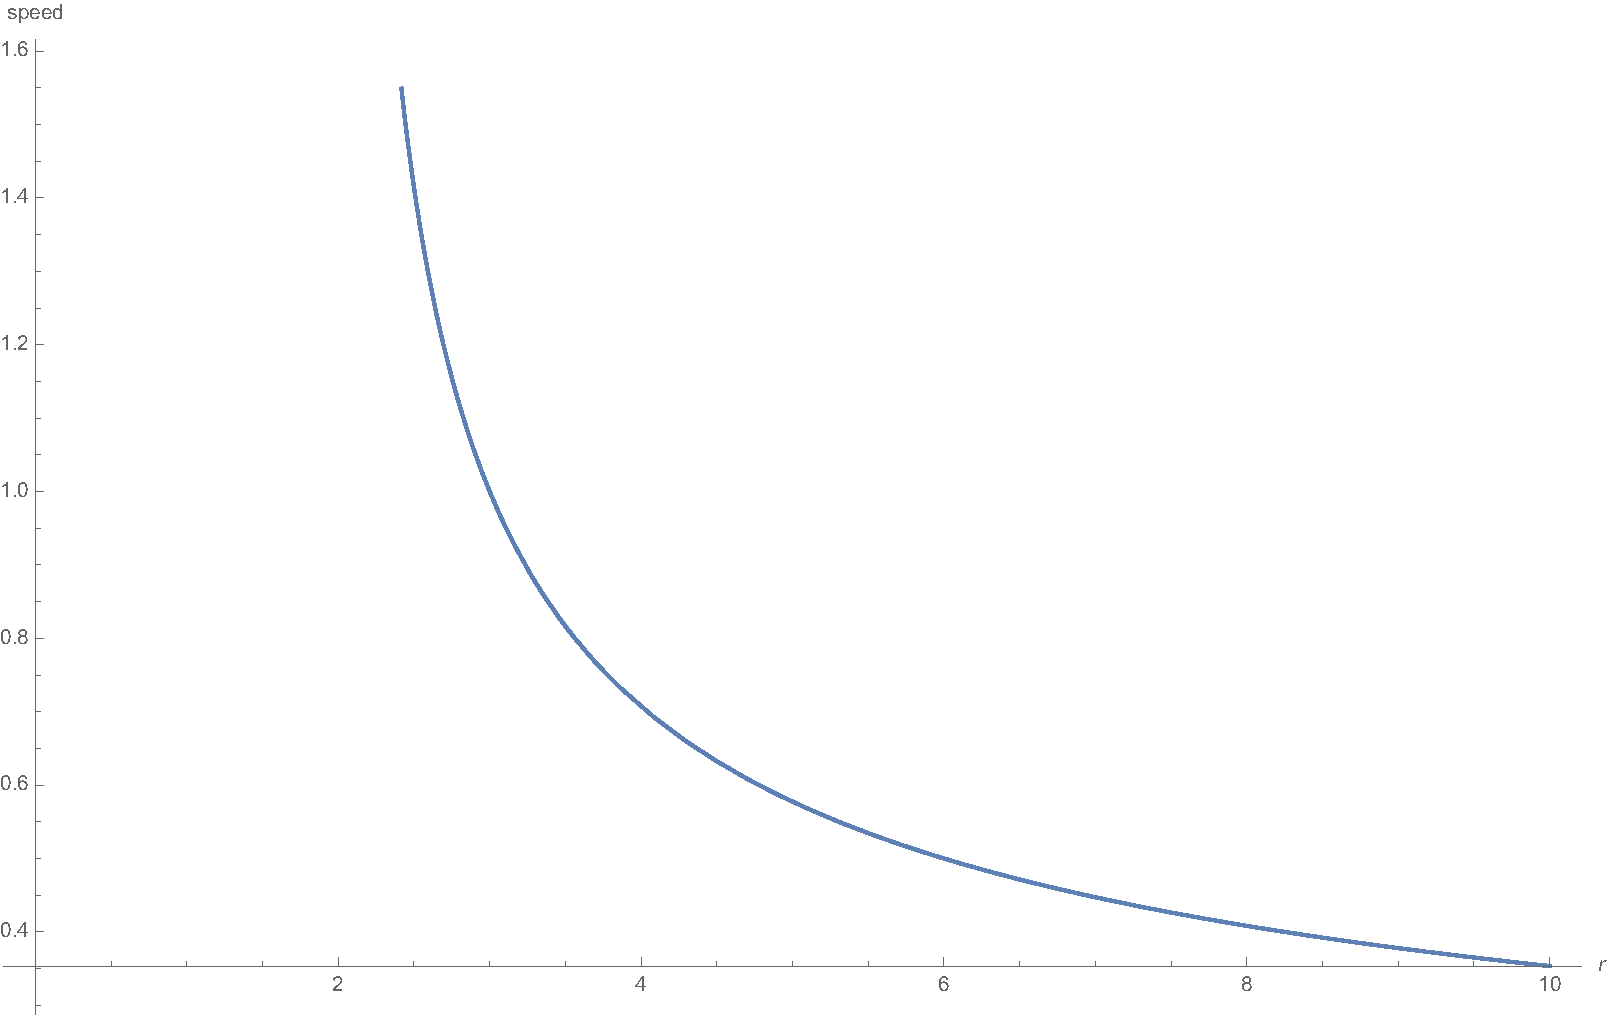
\includegraphics[width=.8\columnwidth]{speed}
            \caption{Speed as measured by a shell observer (as a function of r)}
            \label{fig:speed}
          \end{figure}
          
          \noindent Plugging in the value of $r=6m$ gives a speed of
          \begin{align}
            v &= \frac{1}{\sqrt{1-\frac{2m}{6m}}}\frac{m\sqrt{6}}{6m} \\
              &= \frac{1}{\sqrt{1-\frac{1}{3}}}\frac{\sqrt{6}}{6}\\
              &= \frac{\sqrt{3}}{\sqrt{2}}\frac{\sqrt{3}\sqrt{2}}{6} \\
            &= \frac{3}{6} = \frac{1}{2}
          \end{align}
          So the speed for an object of radius $6m$ is $0.5c$! That's pretty fast!
        \end{solution}

      \item Is a circular orbit at $r=\frac{5}{2}m$ possible?
        \begin{solution}
          As we discussed in class, for circular orbits we must have that
          $dV/dr=0$. This enables us to conclude that
          \begin{align}
            V' &= \frac{1}{r^4}\left( mr^2-\ell^2r+3m\ell^2 \right) = 0 \\
            \Rightarrow r &= \frac{\ell}{2}\left( \frac{\ell}{m}\pm\sqrt{\frac{\ell^2}{m^2}-12} \right)
          \end{align}
          This radius is only well defined for non-negative values of the
          radical. That is, stable circular orbits must satisfy
          \begin{equation}
            \ell^2\geq 12m^2
          \end{equation}
         given that the angular momentum (per mass) $\ell$ is directly related
         to $r$ for circular orbits by equation (15), we have that
         \begin{align}
           \ell^2 &= \frac{mr}{1-\frac{3m}{r}} = \frac{\frac{5}{2}m^2}{1-\frac{3m}{\frac{5}{2}m}} \\
                  &= -\frac{25}{2}m^2 < 12m^2
         \end{align}
         Therefore, an object of radius $r=\frac{5}{2}m$ does not satisfy (25),
         and so we do not expect a circular orbit of this radius to exist.
        \end{solution}
        
      \item Determine the smallest radius at which a circular orbit is possible,
        and the (shell) speed of a satellite in such an orbit.

        \begin{solution}
          As mentioned in (b), to have a stable orbit, an object must satisfy
          the relationship given by equation (25). Therefore, to find the
          smallest possible orbit, we can take the equality and then solve for
          the radius, i.e. $\ell^2 = 12m^2$
          \begin{align}
            r &= \frac{\ell}{2}\left( \frac{\ell}{m}\pm\sqrt{\frac{\ell^2}{m^2}-12} \right)\\
              &= \frac{\ell^2}{2m} \\
            &= \frac{12m^2}{2m} = 6m
          \end{align}
          after checking with Wikipedia, it appears that this solution does
          agree with the $r_{isco}$ radius (innermost stable circular orbit) \url{https://en.wikipedia.org/wiki/Innermost_stable_circular_orbit}. An
          object at this radius would have a speed of $0.5c$ which is exactly
          what we found for part (a)!\\
          
        \end{solution}
        
    \end{enumerate}

  \item \textbf{NULL ORBITS}\\
    Imagine a beam of light in orbit around a Schwarzschild black hole at
    constant radius. 
    \begin{enumerate}[leftmargin=2em, label=(\textbf{\alph*})]
      \item How fast would a shell observer think the beam of light is
        traveling? \\
        \noindent\textit{Your answer must be supported by an explicit
          calculation}

        \begin{solution}
          The length of any lightlike trajectory must be zero, therefore, $ds=0$
          and consequently our line element may be simplified.
          \begin{equation}
            0 = -\left( 1-\frac{2m}{r} \right)dt^2+r^2d\phi^2
          \end{equation}
          where I have again set $dr=0$ for a circular orbit. As we mentioned
          earlier, a shell observer measures distance on a shell as $rd\phi$ and
          therefore, we can try and solve the above for the speed as
          $rd\phi/dt$.
          \begin{align}
            \frac{r^2d\phi^2}{dt^2} &= \left( 1-\frac{2m}{r} \right) \\
           \Rightarrow \frac{rd\phi}{dt}  &= \pm\sqrt{ 1-\frac{2m}{r} }
          \end{align}
          This is really cool! From this perspective, as an object approaches
          the Schwarzschild radius, it appears to \textit{slow down}! This also
          agrees with what an observer far away should observe: for large r,
          the speed is approximately $1c$. I am tempted to leave this answer as
          is but special relativity suggests that the speed of light should be
          constant in all intertial frames. Here we don't have inertial frames
          but rather \textit{the laws of physics are the same for all
            observers in free-fall}. How do we resolve this? I think that the
          answer lies in the fact that while the light is moving in
          ``free-fall'', our ``shell-observer'' is not; the shell observer is
          stationary and measures time using proper time as we already decided
          in equation (5). Therefore, the speed of the light \textit{as measured
            by the shell observer} is
          \begin{equation}
            \frac{rd\phi}{d\tau} =\pm \frac{\sqrt{1-\frac{2m}{r}}}{\sqrt{1-\frac{2m}{r}}} = \pm 1
          \end{equation}
          As we would hope, the shell observer measures the light moving at the
          speed of light! I am still really confused about this... The answer is
          either (33) or (34). Hopefully we can resolve this in class.\\
        \end{solution}
        

    \item How fast would an observer far away think the beam of light is
      traveling?\\
      \noindent\textit{Recall that observers far away believe that $t$ and $r$
      have their usual properties from special relativity. They are not really
      ``observers'' so much as ``bookkeepers''.}\\
      \begin{solution}
        As the hint mentions, a far away bookkeeper experiences regular
        Minkowski flat spacetime. Therefore, they measure distance as something
        more like
        \begin{align}
          ds^2 = d\ell^2-dt^2
        \end{align}
        Here, a lightlike trajectory still must have zero length, and therefore,
        measures the speed as
        \begin{align}
          0 &= d\ell^2-dt^2 \\
          \Rightarrow \frac{d\ell}{dt} &=  1
        \end{align}
        In other words, the distance observer measures the light to travel at
        the speed of light $c$, in agreement with the second postulate of
        special relativity. \\
      \end{solution}


    \item At what value(s) of $r$, if any, is such an orbit possible? \\
      \begin{solution}
        If we begin with equations (8), and (9), we can combine them with (31)
        but instead keeping the $dr$ term. This gives us the third geodesic
        equation but for Null orbits specifically.
        \begin{equation}
          \dot r^2 = e^2-\frac{\ell^2}{r^2}+\frac{2m\ell^2}{r^3}
        \end{equation}
        Differentiating this equation and dividing through by $\dot r$ yields
        \begin{equation}
          \ddot r = \frac{\ell^2}{r^3}-\frac{3m\ell^2}{r^4} = \frac{\ell^2}{r^3}\left( 1-\frac{3m}{r} \right)
        \end{equation}
        For circular orbits, the condition that $V'=0$ implies that $\ddot r = 0$. Therefore, we have
        that light in a circular orbit around a black hole of mass $m$ has a
        radius
        \begin{equation}
          r = 3m = \frac{3}{2}\;r_s
        \end{equation}
        after searching the internet, it appears that my solution agrees with
        the accepted value for the radius of the \textit{photon sphere} around a
        Schwarzschild black hole
        \url{https://en.wikipedia.org/wiki/Photon_sphere}. 
      \end{solution}
      
        
        
    \end{enumerate}
    
    

\end{enumerate}

 
\end{document}






























